\section{Vectores en $\rn$}

\subsection{}

\begin{frame}\frametitle{Vectores en el plano}

\begin{block}{\textbf{Definición 1}}
	\justifying
	Un \textbf{vector en el plano} se representa geométricamente por un segmento de recta
	dirigido, cuyo \textit{\color{verde} punto inicial} es el origen $(0,0)$ y su \textit{\color{red} punto terminal} 
	es un punto arbitrario $(x_1,x_2)$.
\end{block}

\vspace{0mm}

\begin{center}
	\begin{tikzpicture}[thick,scale=0.8, every node/.style={scale=0.65}]%[scale=.8,font=\scriptsize]
	\draw[help lines,step=5mm,black,dotted] (-4,-2) grid (4,4);
	\draw[thick,-latex] (-4,0) -- (4,0) node[right] {\large $x$};
	\draw[thick,-latex] (0,-2) -- (0,4) node[above] {\large $y$};
	\fill[color=verde,draw] (0,0) circle (2pt); % node[below, left] {$(0,0)$};
	\fill[color=red,draw] (2,3) circle (2pt) node[above, right] {\large $(x_1,x_2)$};
	\fill[color=blue,draw] (1.1,1.5) node[above, right] {\large $\x$};
	\draw [color=blue,->] (0,0) -- (2,3);
	\end{tikzpicture}
\end{center}

\end{frame}

%%------------------------------------------------------------------------------------------------------

\subsection{}

\begin{frame}\frametitle{Ejemplos de vectores en el plano}

\vspace{-2mm}

\begin{figure}	
	\begin{subfigure}[b]{\textwidth}
		\centering
		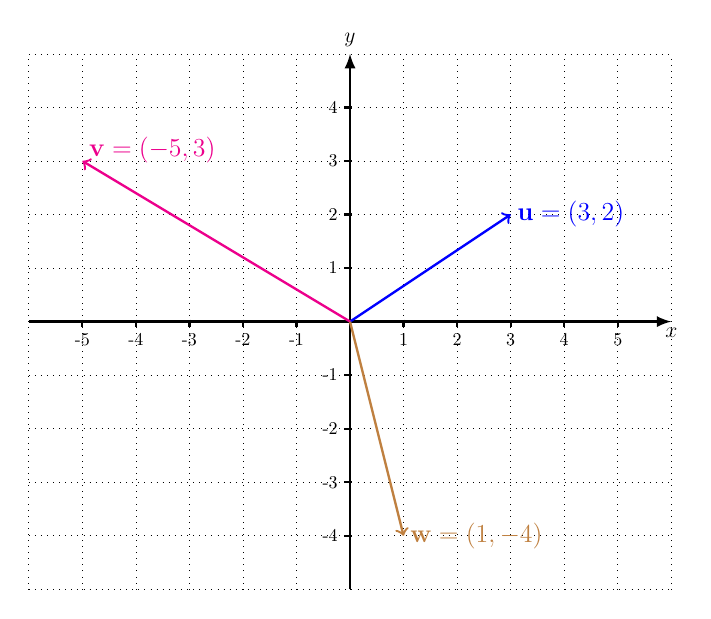
\begin{tikzpicture}[thick,scale=0.68, every node/.style={scale=0.65}]%[scale=.8,font=\scriptsize]
		% axis
		\draw[help lines,black,dotted] (-6,-5) grid (6,5);
		\draw[thick,-latex] (-6,0) -- (6,0) node[below] {\large $x$};
		\draw[thick,-latex] (0,-5) -- (0,5) node[above] {\large $y$};
		% Ticks
		\foreach \x in {1,...,5}
			\draw (\x,1pt) -- (\x,-3pt) 
				node[anchor=north] {\x};
		\foreach \x in {-5,...,-1}
			\draw (\x,1pt) -- (\x,-3pt) 
				node[anchor=north] {\x};		
		\foreach \y in {1,...,4}
			\draw (1pt,\y) -- (-3pt,\y) 
				node[anchor=east] {\y}; 		
		\foreach \y in {-4,...,-1}
			\draw (1pt,\y) -- (-3pt,\y) 
				node[anchor=east] {\y}; 		
		%\fill[color=blue] (0,0) circle[radius=2pt];			
		% Vector u
		\draw [line width=0.3mm,color=blue,->] (0,0) -- (3,2);
		\fill[color=blue,draw] (3,2) node[right] {\Large $\mathbf{u}=(3,2) $};	
		% Vector v
		\draw [line width=0.3mm,color=magenta,->] (0,0) -- (-5,3);
		\fill[color=magenta,draw] (-5,3.2) node[right] {\Large $\mathbf{v}=(-5,3) $};	
		% Vector w
		\draw [line width=0.3mm,color=brown,->] (0,0) -- (1,-4);
		\fill[color=brown,draw] (1,-4) node[right] {\Large $\mathbf{w}=(1,-4) $};	
		% Vector lambda v
%		\draw [line width=0.2mm,color=red,->] (0,0) -- (2.5,1.67);
%		\fill[color=red,draw] (2.5,1.5) node[below] {\Large $\lambda\mathbf{v} $};	
		\end{tikzpicture}
		\caption{Ejemplo 1}
	\end{subfigure}
%	\caption{Pictures of animals}\label{fig:animals}
\end{figure}

\end{frame}

%------------------------------------------------------------------------------------------------------

\subsection{}

\begin{frame}%\frametitle{Suma de vectores en el plano}

\vspace{-1mm}

\begin{block}{\textbf{Definición 2 (Igualdad de vectores)}}
	\justifying
	Dos vectores $\mathbf{u}=(u_1,u_2)$ y $\mathbf{v}=(v_1,v_2)$ en el plano se dice que son \textit{iguales}
	si y sólo si $u_1=v_1$ y $u_2=v_2$.
\end{block}

\vspace{-1mm}

\begin{block}{\textbf{Definición 3 (Suma de vectores en el plano)}}
	\justifying
	Sean $\mathbf{u}=(u_1,u_2)$ y $\mathbf{v}=(v_1,v_2)$ vectores en el plano.
	La \textbf{suma} de $\mathbf{u}$ y $\mathbf{v}$ se define como el vector
	\[
	\mathbf{u+v} = (u_1,u_2) + (v_1,v_2) = (u_1+v_1,u_2+v_2)
	\]
\end{block}

\begin{figure}	
	\begin{subfigure}[b]{0.45\textwidth}
		\centering
		\begin{tikzpicture}[thick,scale=0.4, every node/.style={scale=0.6}]%[scale=.8,font=\scriptsize]
		% axis
		\draw[help lines,black,dotted] (-5,-3) grid (5,5);
		\draw[thick,-latex] (-5,0) -- (5,0) node[below] {\large $x$};
		\draw[thick,-latex] (0,-3) -- (0,5) node[above] {\large $y$};
		% Ticks
		\foreach \x in {1,...,4}
			\draw (\x,1pt) -- (\x,-3pt) node[anchor=north] {\x};
		\foreach \x in {-4,...,-1}		
			\draw (\x,1pt) -- (\x,-3pt) node[anchor=north] {\x};	
		\foreach \y in {1,...,4}
			\draw (1pt,\y) -- (-3pt,\y) node[anchor=east] {\y}; 		
		\foreach \y in {-2,...,-1}
			\draw (1pt,\y) -- (-3pt,\y) node[anchor=east] {\y}; 			
		%\fill[color=blue] (0,0) circle[radius=2pt];			
		% Vector u
		\fill[color=blue,draw] (3,1) circle (3pt) node[right] {$(3,1)$};
		\draw [line width=0.2mm,color=blue,->] (0,0) -- (3,1);
		\fill[color=blue,draw] (1.5,0.3) node[below,right] {$\u $};
		% Vector v
		\fill[color=blue,draw] (1,3) circle (3pt) node[above] {$(1,3)$};
		\draw [line width=0.2mm,color=blue,->] (0,0) -- (1,3);
		\fill[color=blue,draw] (0.55,1.8) node[above,right] { $\v $};	
		% Vector lambda u+v
		\fill[color=red,draw] (4,4) circle (3pt) node[above] {$(4,4)$};
		\draw [line width=0.2mm,color=red,->] (0,0) -- (4,4);
		\fill[color=red,draw] (2,2) node[rotate=45,below] { $\u+\v $};	
		% Paralelogramo
		\draw [line width=0.1mm,color=cyan,dashed,-] (1,3) -- (4,4);
		\draw [line width=0.1mm,color=cyan,dashed,-] (3,1) -- (4,4);
		\end{tikzpicture}
		\caption{Ejemplo 2}
	\end{subfigure}
	\hfill
	\begin{subfigure}[b]{0.45\textwidth}
		\centering
		\begin{tikzpicture}[thick,scale=0.4, every node/.style={scale=0.6}]%[scale=.8,font=\scriptsize]
		% axis
		\draw[help lines,black,dotted] (-5,-3) grid (5,5);
		\draw[thick,-latex] (-5,0) -- (5,0) node[below] {\large $x$};
		\draw[thick,-latex] (0,-3) -- (0,5) node[above] {\large $y$};
		% Ticks
		\foreach \x in {1,...,4}
		\draw (\x,1pt) -- (\x,-3pt) node[anchor=north] {\x};
		\foreach \x in {-4,...,-1}		
		\draw (\x,1pt) -- (\x,-3pt) node[anchor=north] {\x};	
		\foreach \y in {1,...,4}
		\draw (1pt,\y) -- (-3pt,\y) node[anchor=east] {\y}; 		
		\foreach \y in {-2,...,-1}
		\draw (1pt,\y) -- (-3pt,\y) node[anchor=east] {\y}; 			
		%\fill[color=blue] (0,0) circle[radius=2pt];			
		% Vector u
		\fill[color=blue,draw] (1,4) circle (3pt) node[above] {$(1,4)$};
		\draw [line width=0.2mm,color=blue,->] (0,0) -- (1,4);
		\fill[color=blue,draw] (0.6,2.5) node[below,right] {$\u $};
		% Vector v
		\fill[color=blue,draw] (2,-2) circle (3pt) node[below,right] {$(2,-2)$};
		\draw [line width=0.2mm,color=blue,->] (0,0) -- (2,-2);
		\fill[color=blue,draw] (1,-1) node[above,right] { $\v $};	
		% Vector lambda u+v
		\fill[color=red,draw] (3,2) circle (3pt) node[above,right] {$(3,2)$};
		\draw [line width=0.2mm,color=red,->] (0,0) -- (3,2);
		\fill[color=red,draw] (1.3,1.7) node[rotate=33,below] { $\u+\v $};	
		% Paralelogramo
		\draw [line width=0.12mm,color=cyan,dashed,-] (1,4) -- (3,2);
		\draw [line width=0.12mm,color=cyan,dashed,-] (2,-2) -- (3,2);
		\end{tikzpicture}
		\caption{Ejemplo 3}
	\end{subfigure}
	%	\caption{Pictures of animals}\label{fig:animals}
\end{figure}

\end{frame}

%------------------------------------------------------------------------------------------------------

\subsection{}

\begin{frame}\frametitle{Multiplicación escalar}


\begin{block}{\textbf{Definición 4 (Multiplicación por escalar)}}
	\justifying
	Sea $\mathbf{v}=(v_1,v_2)$ un vector en el plano y $c$ un escalar.
	La \textbf{multiplicación por escalar}  de un vector $\mathbf{v}$ por el escalar $c$ se define como el vector
	\[
	c\mathbf{v} = c(v_1,v_2) = (cv_1,cv_2)
	\]	
\end{block}

\begin{figure}	
	\begin{subfigure}[b]{0.45\textwidth}
		\centering
		\begin{tikzpicture}[scale=0.4, every node/.style={scale=0.6}]%[scale=.8,font=\scriptsize]
		% axis
		\draw[help lines,black,dotted] (-5,-5) grid (5,5);
		\draw[thick,-latex] (-5,0) -- (5,0) node[below] {\large $x$};
		\draw[thick,-latex] (0,-5) -- (0,5) node[above] {\large $y$};
		% Ticks
		\foreach \x in {1,...,4}
		\draw (\x,1pt) -- (\x,-3pt) node[anchor=north] {\x};
		\foreach \x in {-4,...,-1}		
		\draw (\x,1pt) -- (\x,-3pt) node[anchor=north] {\x};	
		\foreach \y in {1,...,4}
		\draw (1pt,\y) -- (-3pt,\y) node[anchor=east] {\y}; 		
		\foreach \y in {-4,...,-1}
		\draw (1pt,\y) -- (-3pt,\y) node[anchor=east] {\y}; 			
		%\fill[color=blue] (0,0) circle[radius=2pt];			
		% Vector v
		\fill[color=blue,draw] (2,1) circle (3pt) node[below] {\hspace{3mm} $(2,1)$};
		\draw [line width=0.4mm,color=blue,->] (0,0) -- (2,1);
		\fill[color=blue,draw] (0.8,1) node[below] {$\v $};
		% Vector cv
		\fill[color=red,draw] (4,2) circle (3pt) node[above,right] {$(4,2)$};
		\draw [line width=0.2mm,color=red,->] (0,0) -- (4,2);
		\fill[color=red,draw] (2.2,1.7) node[above,right] { $2\v $};	
		\end{tikzpicture}
		\caption{Ejemplo 4}
	\end{subfigure}
	\hfill
	\begin{subfigure}[b]{0.45\textwidth}
		\centering
		\begin{tikzpicture}[scale=0.4, every node/.style={scale=0.6}]%[scale=.8,font=\scriptsize]
		% axis
		\draw[help lines,black,dotted] (-5,-5) grid (5,5);
		\draw[thick,-latex] (-5,0) -- (5,0) node[below] {\large $x$};
		\draw[thick,-latex] (0,-5) -- (0,5) node[above] {\large $y$};
		% Ticks
		\foreach \x in {1,...,4}
		\draw (\x,1pt) -- (\x,-3pt) node[anchor=north] {\x};
		\foreach \x in {-4,...,-1}		
		\draw (\x,1pt) -- (\x,-3pt) node[anchor=north] {\x};	
		\foreach \y in {1,...,4}
		\draw (1pt,\y) -- (-3pt,\y) node[anchor=east] {\y}; 		
		\foreach \y in {-4,...,-1}
		\draw (1pt,\y) -- (-3pt,\y) node[anchor=east] {\y}; 			
		%\fill[color=blue] (0,0) circle[radius=2pt];			
		% Vector v
		\fill[color=blue,draw] (2,1) circle (3pt) node[below,right] {$(2,1)$};
		\draw [line width=0.4mm,color=blue,->] (0,0) -- (2,1);
		\fill[color=blue,draw] (0.8,1) node[below] {$\v $};
		% Vector cv
		\fill[color=red,draw] (-4,-2) circle (3pt) node[below] {$(-4,-2)$};
		\draw [line width=0.2mm,color=red,->] (0,0) -- (-4,-2);
		\fill[color=red,draw] (-3.6,-1) node[above,right] { $-2\v $};	
		\end{tikzpicture}
		\caption{Ejemplo 5}
	\end{subfigure}
	%	\caption{Pictures of animals}\label{fig:animals}
\end{figure}

\end{frame}

%%------------------------------------------------------------------------------------------------------

\subsection{}

{\nologo
\begin{frame}\frametitle{Operaciones con vectores en el plano}

\begin{block}{}%{\textbf{Definición 3 (Operaciones con vectores)}}
	\justifying
	Sean $\mathbf{u}=(u_1,u_2)$ y $\mathbf{v}=(v_1,v_2)$ vectores en el plano y $c\in\r$ un escalar.
	\begin{enumerate}
		\item La \textbf{suma} de $\mathbf{u}$ y $\mathbf{v}$ se define como el vector
		\[
		\mathbf{u+v} = (u_1,u_2) + (v_1,v_2) = (u_1+v_1,u_2+v_2)
		\]
		\item La \textbf{multiplicación por escalar} de un vector $\mathbf{v}$ por un escalar $c$ se define como el vector
		\[
		c\mathbf{v} = c(v_1,v_2) = (cv_1,cv_2)
		\]	
	\end{enumerate}
\end{block}

\begin{ej}{\textbf{Ejemplo 6}}
	Considere los vectores $\mathbf{u}=(3,4)$ y $\mathbf{v}=(-2,5)$. Calcule:
	
	\vspace{-2mm}
	\begin{multicols}{3}
		\begin{enumerate}
			\item[\labelname{$a$}] $\frac{1}{2}\v$.
			\item[\labelname{$b$}] $\u-\v$.
			\item[\labelname{$c$}] $\frac{1}{2}\v+\u$.
		\end{enumerate}
	\end{multicols}
	
	\vspace{-2mm}
\end{ej}

\end{frame}
}
	
%------------------------------------------------------------------------------------------------------

\subsection{} 

{\nologo
\begin{frame}\frametitle{Vectores en el plano}

\begin{prop}{\textbf{Propiedad 1}}
	Sean $\mathbf{u}, \mathbf{v}$ y $\mathbf{w}$ vectores en el plano y sean $c$ y $d$ escalares. Entonces:
	\begin{multicols}{2}		
		\begin{enumerate}			
			\justifying
			\item $\mathbf{u}+\mathbf{v}$ es un vector en el plano. \\[4mm]			
			\item $\mathbf{u}+\mathbf{v} = \mathbf{v}+\mathbf{u}$. \\[3mm]			
			\item $(\mathbf{u}+\mathbf{v})+\mathbf{w} = \mathbf{u}+(\mathbf{v}+\mathbf{w})$. \\[4mm]			
			\item El vector cero $\mathbf{0}=(0,0)$ satisface la siguiente propiedad:
			\[
			\mathbf{u}+\mathbf{0} = \mathbf{u}
			\]
			
			\vspace{2mm}	
			\item El vector $-\mathbf{u}=(-u_1,-u_2)$ satisface la siguiente propiedad:
			\[
			\mathbf{u}+(-\mathbf{u}) = \mathbf{0}
			\]	
			\columnbreak
			\item $c\mathbf{u}$ es un vector en el plano. \\[4mm]			
			\item $c(\mathbf{u}+\mathbf{v}) = c\mathbf{u} + c\mathbf{v}$. \\[3mm]
			\item $(c+d)\mathbf{u} = c\mathbf{u} + d\mathbf{u}$ \\[4mm]
			\item $c(d\mathbf{u}) = (cd)\mathbf{u}$ \\[1.3cm]
			\item $1\mathbf{u} = \mathbf{u}$.
		\end{enumerate}		
	\end{multicols}
\end{prop}

\end{frame}
}

%------------------------------------------------------------------------------------------------------

\subsection{}

{\nologo
\begin{frame}\frametitle{Vectores en $\rn$}

\vspace{-3mm}
\begin{alertblock}{\textbf{Observación 1}}
	\begin{enumerate}
		\item[\labelname{$a$}] El producto de un vector $\mathbf{v}$ por el escalar $-1$ se denota por
		\[
		-\mathbf{v} = (-1)\mathbf{v}.
		\]
		
		\vspace{0mm}	
		\item[\labelname{$b$}] Al vector $-\mathbf{v}$ se le denomina \textit{inverso aditivo} de $\mathbf{v}$.
		
		\vspace{2mm}	
		\item[\labelname{$c$}] La resta de $\mathbf{u}$ y $\mathbf{v}$ se se define como 
		$\mathbf{u}-\mathbf{v} = \mathbf{u} + (-\mathbf{v}) $.

		\vspace{2mm}	
		\item[\labelname{$d$}] Al conjunto de todos los puntos $\x = (x_1,x_2)$ en el plano se le denota por 
		\[
		\r^2 = \{ (x_1,x_2) \mid x_1 \ \mbox{y} \  x_2 \in \r \}
		\]
%		\item Se dice que $\r^2$ es un espacio vectorial (real).

		\vspace{1mm}	
		\item[\labelname{$e$}] Al conjunto de todos los puntos $\x = (x_1,x_2,x_3)$ en el espacio se le denota por 
		\[
		\r^3 = \{ (x_1,x_2,x_3) \mid x_1, x_2 \ \mbox{y} \  x_2 \in \r \}
		\]

		\vspace{2mm}	
		\item[\labelname{$f$}] Al conjunto de todas las $n$-túplas $\x = (x_1,\hdots, x_n)$ se le denota por 
		\[
		\rn = \{ (x_1,\hdots, x_n) \mid x_1, \hdots, x_n \in \r \}
		\]
	\end{enumerate}
\end{alertblock}

\end{frame}
}

%------------------------------------------------------------------------------------------------------

\subsection{}

{\nologo
\begin{frame}%\frametitle{Vectores en el plano}

\vspace{-2mm}
\begin{block}{\textbf{Definición 5 (Operaciones con vectores en $\r^n$)}}
	\justifying
	Sean $\mathbf{u}=(u_1,\hdots,u_n)$ y $\mathbf{v}=(v_1,\hdots,v_n)$ vectores en $\r^n$ y $c\in\r$ un escalar.
	\begin{enumerate}
		\item La \textbf{suma} de $\mathbf{u}$ y $\mathbf{v}$ se define como el vector
		\[
		\mathbf{u+v} = (u_1,\hdots,u_n) + (v_1,\hdots,v_n) = (u_1+v_1,\hdots,u_n+v_n)
		\]
		\item La \textbf{multiplicación por escalar} de un vector $\mathbf{v}$ por un escalar $c$ se define como el vector
		\[
		c\mathbf{v} = c(v_1,\hdots,v_n) = (cv_1,\hdots,cv_n)
		\]	
	\end{enumerate}
\end{block}

\vspace{-2mm}
\begin{alertblock}{\textbf{Observación 2}}
	\begin{enumerate}
		\item[\labelname{$a$}] El producto de un vector $\mathbf{v}$ por el escalar $-1$ se denota por
		\[
		-\mathbf{v} = (-1)\mathbf{v} = (-v_1,\hdots,-v_n).
		\]
		\item[\labelname{$b$}] Al vector $-\mathbf{v}$ se le denomina \textit{inverso aditivo} de $\mathbf{v}$.
		\item[\labelname{$c$}] La resta de $\mathbf{u}$ y $\mathbf{v}$ se se define como 
			\[
				\mathbf{u}-\mathbf{v} = \mathbf{u} + (-\mathbf{v}) =  (u_1-v_1,\hdots,u_n-v_n).
			\]
		\item[\labelname{$b$}] El vector cero en $\r^n$ se denota por  $\mathbf{0} = (0,\hdots,0)$.
	\end{enumerate}
\end{alertblock}

\vspace{0mm}

\end{frame}
}

%%------------------------------------------------------------------------------------------------------

\subsection{}

{\nologo
\begin{frame}\frametitle{Operaciones con vectores en $\rn$}

\begin{block}{\textbf{Definición 5 (Operaciones con vectores en $\r^n$)}}
	\justifying
	Sean $\mathbf{u}=(u_1,\hdots,u_n)$ y $\mathbf{v}=(v_1,\hdots,v_n)$ vectores en $\r^n$ y $c\in\r$ un escalar.
	\begin{enumerate}
		\item La \textbf{suma} de $\mathbf{u}$ y $\mathbf{v}$ se define como el vector
		\[
		\mathbf{u+v} = (u_1,\hdots,u_n) + (v_1,\hdots,v_n) = (u_1+v_1,\hdots,u_n+v_n)
		\]
		\item La \textbf{multiplicación por escalar} de un vector $\mathbf{v}$ por un escalar $c$ se define como el vector
		\[
		c\mathbf{v} = c(v_1,\hdots,v_n) = (cv_1,\hdots,cv_n)
		\]	
	\end{enumerate}
\end{block}

\begin{ej}{\textbf{Ejemplo 7}}
	Considere los vectores $\mathbf{u}=(-1,0,1)$ y $\mathbf{v}=(2,-1,5)$. Calcule:
	
	\vspace{-2mm}
	\begin{multicols}{3}
		\begin{enumerate}
			\item[\labelname{$a$}] $\u+\v$.
			\item[\labelname{$b$}] $2\u$.
			\item[\labelname{$c$}] $\v-2\u$.
		\end{enumerate}
	\end{multicols}
	
	\vspace{-2mm}
\end{ej}

\end{frame}
}

%%------------------------------------------------------------------------------------------------------

\subsection{} 

{\nologo
\begin{frame}\frametitle{Vectores en $\r^n$}


\begin{prop}{\textbf{Propiedad 2}}
	Sean $\mathbf{u}, \mathbf{v}$ y $\mathbf{w}$ vectores en $\r^n$ y sean $c$ y $d$ escalares. Entonces:
	\begin{multicols}{2}		
		\begin{enumerate}			
			\justifying
			\item $\mathbf{u}+\mathbf{v}$ es un vector en $\r^n$. \\[4mm]			
			\item $\mathbf{u}+\mathbf{v} = \mathbf{v}+\mathbf{u}$. \\[3mm]			
			\item $(\mathbf{u}+\mathbf{v})+\mathbf{w} = \mathbf{u}+(\mathbf{v}+\mathbf{w})$. \\[4mm]			
			\item El vector cero $\mathbf{0}=(0,\hdots,0)$ satisface la siguiente propiedad:
			\[
			\mathbf{u}+\mathbf{0} = \mathbf{u}
			\]
			
			\vspace{2mm}	
			\item El vector $-\mathbf{u}=(-u_1,\hdots,-u_n)$ satisface la siguiente propiedad:
			\[
			\mathbf{u}+(-\mathbf{u}) = \mathbf{0}
			\]	
			\columnbreak
			\item $c\mathbf{u}$ es un vector en $\r^n$. \\[4mm]			
			\item $c(\mathbf{u}+\mathbf{v}) = c\mathbf{u} + c\mathbf{v}$. \\[3mm]
			\item $(c+d)\mathbf{u} = c\mathbf{u} + d\mathbf{u}$ \\[4mm]
			\item $c(d\mathbf{u}) = (cd)\mathbf{u}$ \\[1.3cm]
			\item $1\mathbf{u} = \mathbf{u}$.
		\end{enumerate}		
	\end{multicols}
\end{prop}

\end{frame}
}

%%------------------------------------------------------------------------------------------------------

\subsection{}

{\nologo
\begin{frame}\frametitle{Operaciones con vectores en $\rn$}

\begin{prop}{\textbf{Propiedad 2}}
	Sean $\mathbf{u}, \mathbf{v}$ y $\mathbf{w}$ vectores en $\r^n$ y sean $c$ y $d$ escalares. Entonces:
	
	\vspace{-2mm}
	\begin{multicols}{2}		
		\begin{enumerate}			
			\justifying
			\item $\mathbf{u}+\mathbf{v}$ es un vector en $\r^n$. %\\[4mm]			
			\item $\mathbf{u}+\mathbf{v} = \mathbf{v}+\mathbf{u}$. %\\[3mm]			
			\item $(\mathbf{u}+\mathbf{v})+\mathbf{w} = \mathbf{u}+(\mathbf{v}+\mathbf{w})$. %\\[4mm]			
			\item $\mathbf{u}+\mathbf{0} = \mathbf{u}$.
			\item $\mathbf{u}+(-\mathbf{u}) = \mathbf{0}$.
			
			\columnbreak
			\item $c\mathbf{u}$ es un vector en $\r^n$. %\\[4mm]			
			\item $c(\mathbf{u}+\mathbf{v}) = c\mathbf{u} + c\mathbf{v}$. %\\[3mm]
			\item $(c+d)\mathbf{u} = c\mathbf{u} + d\mathbf{u}$ %\\[4mm]
			\item $c(d\mathbf{u}) = (cd)\mathbf{u}$ %\\[1.3cm]
			\item $1\mathbf{u} = \mathbf{u}$.
		\end{enumerate}		
	\end{multicols}

	\vspace{-2mm}
\end{prop}

\begin{ej}{\textbf{Ejemplo 8}}\justifying
	Considere los vectores $\u=(2,-1,5,0)$, $\v=(4,3,1,-1)$ y $\w=(-6,2,0,3)$. 
	En cada uno de los siguientes casos halle a $\x$.
	
	\vspace{-2mm}
	\begin{multicols}{2}
		\begin{enumerate}
			\item[\labelname{$a$}] $\x = 2\u - (\v+3\w)$.
			\item[\labelname{$b$}] $3(\x+\w) = 2\u - \v + \x$.
		\end{enumerate}
	\end{multicols}
	
	\vspace{-2mm}
\end{ej}

\end{frame}
}

%------------------------------------------------------------------------------------------------------

\subsection{}

\begin{frame}\frametitle{Propiedades de vector cero y del inverso aditivo}

\begin{prop}{\textbf{Propiedad 3}}
	\justifying
	Sean $\mathbf{v}$ un vector en $\r^n$ y $c$ un escalar. Entonces:
	\begin{enumerate}
		\item Si $\mathbf{v}+\mathbf{u}=\mathbf{v}$, entonces $\mathbf{u} = \mathbf{0}$.
		\item Si $\mathbf{v}+\mathbf{u}=\mathbf{0}$, entonces $\mathbf{u} = -\mathbf{v}$.
		\item $0\mathbf{u} = \mathbf{0}$.
		\item $c\mathbf{0} = \mathbf{0}$.
		\item $c\mathbf{u} = \mathbf{0} \ \Longrightarrow \ c=0 \ \ \text{ó} \ \ \mathbf{u} = \mathbf{0}$.
		\item $-(-\mathbf{v}) = \mathbf{v}$.
	\end{enumerate}
\end{prop}

\end{frame}

%%------------------------------------------------------------------------------------------------------

\subsection{}

\begin{frame}\frametitle{Operaciones con vectores en $\rn$}

\begin{ej}{\textbf{Ejemplo 9}}\justifying
	Considere los vectores $\x=(-1,-2,-2)$, $\u=(0,1,4)$, $\v=(-1,1,2)$ y $\w=(3,1,2)$. 
	Encuentre escalares $a, b$ y $c$ tales que
	\[
		\x = a\u + b\v + c\w.
	\]	

\end{ej}

\end{frame}